\scanpage{8}

(B)

\textcircled{$B_1$}
\figure{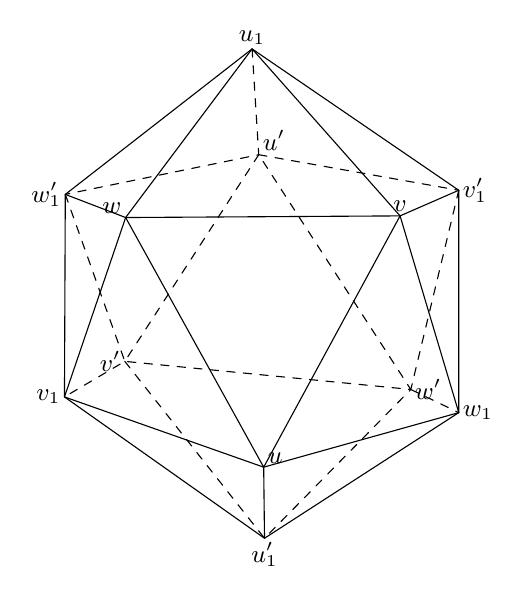
\begin{tikzpicture}[x=0.0105cm,y=-0.0105cm,line cap=round,line join=round,font=\small]
\coordinate (H) at (227,0);
\coordinate (L) at (0,421);
\coordinate (R) at (477,440);
\coordinate (J) at (242,592);
\coordinate (K) at (477,171);
\coordinate (M) at (1,176);
\coordinate (U) at (241,506);
\coordinate (V) at (406,202);
\coordinate (W) at (74,204);
\coordinate (Up) at (235,128);
\coordinate (Vp) at (73,378);
\coordinate (Wp) at (419,412);
\draw[dashed] (H)--(Up)--(M);
\draw[dashed] (Up)--(K);
\draw[dashed] (Up)--(Vp)--(Wp)--cycle;
\draw[dashed] (M)--(Vp)--(L);
\draw[dashed] (Vp)--(J)--(Wp)--(K);
\draw[dashed] (Wp)--(R);
\draw (H)--(M)--(L)--(J)--(R)--(K)--cycle;
\draw (M)--(W)--(V)--(K);
\draw (L)--(W)--(H)--(V)--(R);
\draw (L)--(U)--(R);
\draw (J)--(U);
\draw (W)--(U)--(V);
\node[above,inner sep=1.3pt] at (H) {$u_1$};
\node[left,inner sep=1.3pt] at (L) {$v_1$};
\node[right,inner sep=1.3pt] at (R) {$w_1$};
\node[below,inner sep=1.3pt] at (J) {$u'_1$};
\node[right,inner sep=1.3pt] at (K) {$v'_1$};
\node[left,inner sep=1.3pt] at (M) {$w'_1$};
\node[above right,inner sep=1.3pt] at (U) {$u$};
\node[above,inner sep=1.3pt] at (V) {$v$};
\node[above left,inner sep=1.3pt] at (W) {$w$};
\node[above right,inner sep=1.3pt] at (Up) {$u'$};
\node[left,inner sep=1.3pt] at (Vp) {$v'$};
\node[right,inner sep=1.3pt] at (Wp) {$w'$};
\end{tikzpicture}}

groupe de symétrie $\mathbb Z/2\mathbb Z\times\unsure{\mathfrak S|\mathcal S}_3$ d'ordre $12=120/10$

\uline{NB} $10=20/2$

\figure{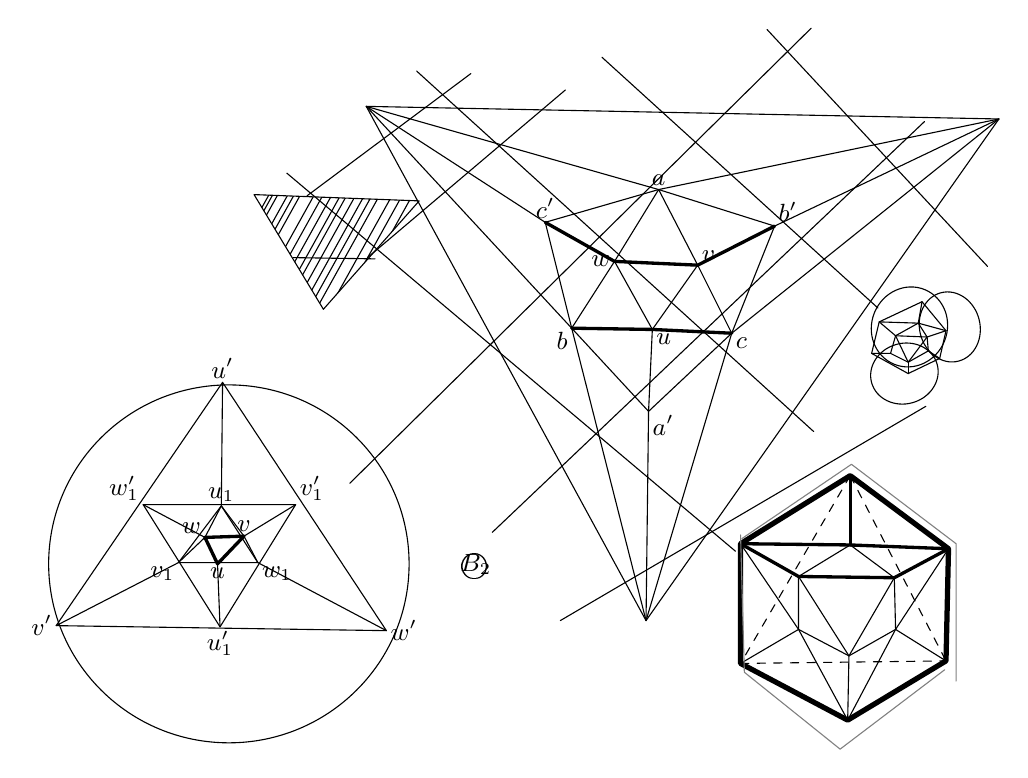
\begin{tikzpicture}[x=0.016cm,y=-0.016cm,line cap=round,line join=round,font=\small]
\coordinate (T) at (246,62);
\coordinate (Q) at (748,72);
\coordinate (Zz) at (468,470);
\coordinate (A) at (478,128);
\coordinate (B) at (409,238);
\coordinate (C) at (536,242);
\coordinate (Ap) at (470,304);
\coordinate (Bp) at (570,157);
\coordinate (Cp) at (388,154);
\coordinate (U) at (473,239);
\coordinate (V) at (509,188);
\coordinate (W) at (443,185);
\coordinate (I) at (157,132);
\coordinate (J) at (288,137);
\coordinate (K) at (212,223);
\coordinate (X) at (188,182);
\coordinate (Y) at (253,183);
\coordinate (H) at (329,36);
\coordinate (Hh) at (199,133);
\coordinate (N) at (404,49);
\coordinate (Nn) at (247,182);
\coordinate (P) at (599,0);
\coordinate (Pp) at (233,361);
\coordinate (Qq) at (689,74);
\coordinate (Qe) at (346,400);
\coordinate (Xx) at (286,34);
\coordinate (Xe) at (601,320);
\coordinate (Yy) at (433,23);
\coordinate (Ye) at (652,222);
\coordinate (Z1) at (564,1);
\coordinate (Z2) at (739,189);
\coordinate (L1) at (183,115);
\coordinate (L2) at (539,415);
\coordinate (Gl) at (400,470);
\coordinate (Gr) at (690,300);
\coordinate (Ht) at (132,281);
\coordinate (Hl) at (0,474);
\coordinate (Hr) at (262,478);
\coordinate (Lt) at (69,378);
\coordinate (Rt) at (190,378);
\coordinate (Bt) at (130,475);
\coordinate (Ut) at (131,379);
\coordinate (Vt) at (97,424);
\coordinate (Wt) at (160,424);
\coordinate (Ui) at (128,425);
\coordinate (Vi) at (149,403);
\coordinate (Wi) at (118,404);
\coordinate (D0) at (630,355);
\coordinate (D1) at (543,409);
\coordinate (D2) at (543,504);
\coordinate (D3) at (628,549);
\coordinate (D4) at (706,502);
\coordinate (D5) at (708,413);
\coordinate (Dt) at (630,410);
\coordinate (F1) at (589,435);
\coordinate (F2) at (665,436);
\coordinate (F3) at (629,498);
\coordinate (F4) at (589,477);
\coordinate (F5) at (666,477);
\coordinate (S0) at (687,217);
\coordinate (S1) at (653,233);
\coordinate (S2) at (647,258);
\coordinate (S3) at (676,274);
\coordinate (S4) at (701,262);
\coordinate (S5) at (706,240);
\coordinate (St) at (684,234);
\coordinate (Si) at (666,244);
\coordinate (Sj) at (691,245);
\coordinate (Sk) at (676,265);
\coordinate (Sl) at (662,258);
\coordinate (Sm) at (692,256);
\coordinate (Badge) at (333,427);
\draw[thin] (T)--(Q)--(Zz)--cycle;
\draw (T)--(Cp);
\draw (T)--(A);
\draw (T)--(B);
\draw (Q)--(A);
\draw (Q)--(Bp);
\draw (Q)--(C);
\draw (Zz)--(Ap);
\draw (Zz)--(B);
\draw (Zz)--(C);
\draw (A)--(Bp)--(C)--(Ap)--(B)--(Cp)--cycle;
\draw[very thick] (Cp)--(W)--(V)--(Bp);
\draw (B)--(W)--(A)--(V)--(C);
\draw[very thick] (B)--(U)--(C);
\draw (Ap)--(U);
\draw (W)--(U)--(V);
\draw[thin] (H)--(Hh);
\draw[thin] (N)--(Nn);
\draw[thin] (P)--(Pp);
\draw[thin] (Qq)--(Qe);
\draw[thin] (Xx)--(Xe);
\draw[thin] (Yy)--(Ye);
\draw[thin] (Z1)--(Z2);
\draw[thin] (L1)--(L2);
\draw[thin] (Gl)--(Gr);
\draw (I)--(J)--(K)--cycle;
\draw[thin] (X)--(Y);
\draw (Ht)--(Hl)--(Hr)--cycle;
\draw (Lt)--(Rt)--(Bt)--cycle;
\draw (Ht)--(Ut);
\draw (Hl)--(Vt);
\draw (Hr)--(Wt);
\draw (Ut)--(Vt)--(Wt)--cycle;
\draw (Bt)--(Ui);
\draw[very thick] (Wi)--(Vi)--(Ui)--cycle;
\draw (Lt)--(Wi)--(Ut)--(Vi)--(Rt);
\draw (Vt)--(Wi);
\draw (Wt)--(Vi);
\draw[line width=1.9pt] (D0)--(D1)--(D2)--(D3)--(D4)--(D5)--cycle;
\draw[very thick] (D1)--(Dt)--(D5);
\draw[very thick] (D0)--(Dt);
\draw[very thick] (D1)--(F1)--(F2)--(D5);
\draw (Dt)--(F1)--(F4)--(D2);
\draw (Dt)--(F2)--(F5)--(D4);
\draw (F1)--(F3)--(F2);
\draw (F4)--(F3)--(F5);
\draw (F3)--(D3);
\draw (D1)--(F4)--(D3)--(F5)--(D5);
\draw[dashed] (D2)--(D4);
\draw[dashed] (D0)--(D2);
\draw[dashed] (D0)--(D4);
\draw (S0)--(S1)--(S2)--(S3)--(S4)--(S5)--cycle;
\draw[thin] (S1)--(St)--(S5);
\draw[thin] (S0)--(St);
\draw[thin] (S1)--(Si)--(Sj)--(S5);
\draw[thin] (St)--(Si)--(Sl)--(S2);
\draw[thin] (St)--(Sj)--(Sm)--(S4);
\draw[thin] (Si)--(Sk)--(Sj);
\draw[thin] (Sl)--(Sk)--(Sm);
\draw[thin] (Sk)--(S3);
\node[above,inner sep=1.3pt] at (A) {$a$};
\node[below left,inner sep=1.3pt] at (B) {$b$};
\node[below right,inner sep=1.3pt] at (C) {$c$};
\node[below right,inner sep=1.3pt] at (Ap) {$a'$};
\node[above right,inner sep=1.3pt] at (Bp) {$b'$};
\node[above,inner sep=1.3pt] at (Cp) {$c'$};
\node[below right,inner sep=1.3pt] at (U) {$u$};
\node[above right,inner sep=1.3pt] at (V) {$v$};
\node[left,inner sep=1.3pt] at (W) {$w$};
\node[above,inner sep=1.3pt] at (Ht) {$u'$};
\node[left,inner sep=1.3pt] at (Hl) {$v'$};
\node[right,inner sep=1.3pt] at (Hr) {$w'$};
\node[above left,inner sep=1.3pt] at (Lt) {$w'_1$};
\node[above right,inner sep=1.3pt] at (Rt) {$v'_1$};
\node[below,inner sep=1.3pt] at (Bt) {$u'_1$};
\node[above,inner sep=1.3pt] at (Ut) {$u_1$};
\node[below left,inner sep=1.3pt] at (Vt) {$v_1$};
\node[below right,inner sep=1.3pt] at (Wt) {$w_1$};
\node[below,inner sep=1.3pt] at (Ui) {$u$};
\node[above,inner sep=1.3pt] at (Vi) {$v$};
\node[above left,inner sep=1.3pt] at (Wi) {$w$};
\node[anchor=center,inner sep=1.3pt] at (Badge) {\textcircled{$B_2$}};
\draw (137,425) ellipse [x radius=143,y radius=142];
\draw[thin] (677,237) ellipse[x radius=30,y radius=32,rotate=-22];
\draw[thin] (709,237) ellipse[x radius=24,y radius=28,rotate=14];
\draw[thin] (673,274) ellipse[x radius=27,y radius=24,rotate=16];
\begin{scope}\clip (I)--(J)--(K)--cycle;
\foreach \t in {152,157,162,167,180,183,187,195,200,205,216,223,230,237,242,249,256,262,268,278,286,294} \draw[thin] (\t,112)--++(-60,108);
\end{scope}
\draw[gray,thin] (543,402)--(546,511)--(622,572)--(705,509);
\draw[gray,thin] (544,405)--(631,346)--(714,409)--(714,518);
\end{tikzpicture}}
% crop-candidate: scan 8

% Left-hand hatched triangle in the preceding TikZ picture.

% Three loops beside the right-hand construction lines.

% Circular projection at lower left of the same picture.

% Heavy hexagon, inner solid and lighter construction strokes at lower right.

% archive sheet number: 7

